\chapter{Source Code Example}
%\label{chapter:title}

\emph{Adding source code to your report/thesis is supported with the package {\normalfont\texttt{listings}}. An example can be found below. Files can be added using {\normalfont\texttt{\textbackslash lstinputlisting[language=<language>]\{<filename>\}}}.}

\begin{lstlisting}[language=Python]
"""
ISA Calculator: import the function, specify the height and it will return a
list in the following format: [Temperature,Density,Pressure,Speed of Sound].
Note that there is no check to see if the maximum altitude is reached.
"""

import math
g0 = 9.80665
R = 287.0
layer1 = [0, 288.15, 101325.0]
alt = [0,11000,20000,32000,47000,51000,71000,86000]
a = [-.0065,0,.0010,.0028,0,-.0028,-.0020]

def atmosphere(h):
    for i in range(0,len(alt)-1):
        if h >= alt[i]:
            layer0 = layer1[:]
            layer1[0] = min(h,alt[i+1])
            if a[i] != 0:
                layer1[1] = layer0[1] + a[i]*(layer1[0]-layer0[0])
                layer1[2] = layer0[2] * (layer1[1]/layer0[1])**(-g0/(a[i]*R))
            else:
                layer1[2] = layer0[2]*math.exp((-g0/(R*layer1[1]))*(layer1[0]-layer0[0]))
    return [layer1[1],layer1[2]/(R*layer1[1]),layer1[2],math.sqrt(1.4*R*layer1[1])]
\end{lstlisting}


\chapter{Latex Tikz Test Code}
\begin{figure}[H]
    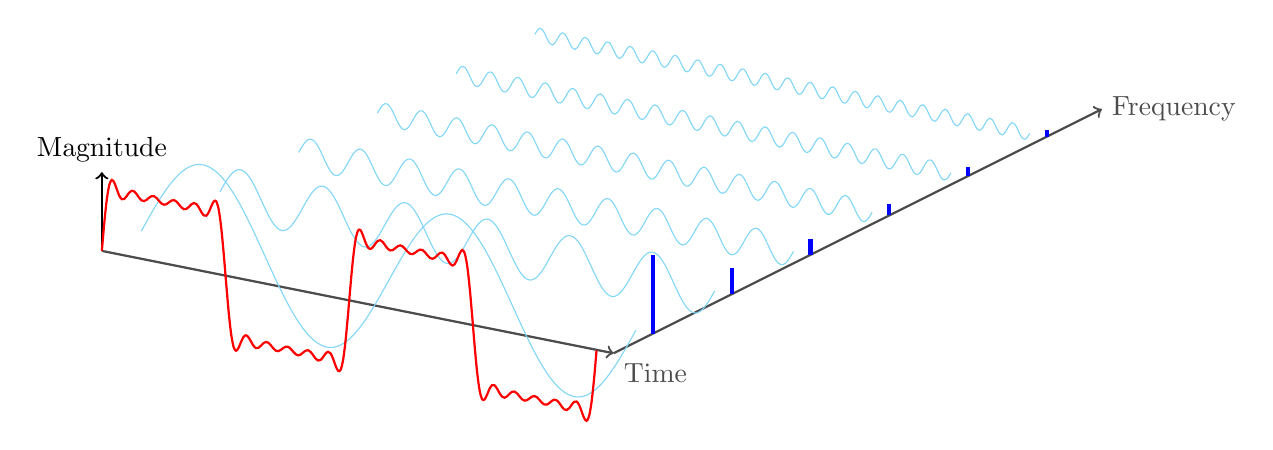
\begin{tikzpicture}[x={(1cm,0.5cm)},z={(0cm,0.5cm)},y={(1cm,-0.2cm)}]%指定坐标系的方向与缩放
        \draw[->,thick,black!70] (0,6.5,0) -- (6.2,6.5,0) node[right] {Frequency}; % 频率轴
        \draw[->,thick,black!70] (0,0,0) -- (0,6.5,0) node[below right] {Time}; % 时间轴
        \draw[->,thick] (0,0,0) -- (0,0,2) node[above] {Magnitude}; 
        
        \foreach \n in {0.5,1.5,...,5.5}{
        \draw [cyan!50, domain=0:2*pi,samples=200,smooth] 
         plot (\n,\x, {sin(4*\n*\x r)/\n });
        \draw[blue, ultra thick] (\n,6.5,0) -- (\n,6.5,1/\n);
        } % 频率逐渐增大振幅逐渐变小的正弦函数
        
        \draw [red, thick, domain=0:2*pi,samples=200,smooth] 
        plot (0,\x, {sin(4*0.5*\x r)/0.5 + sin(4*1.5*\x r)/1.5 + sin(4*2.5*\x r)/2.5
         + sin(4*3.5*\x r)/3.5 + sin(4*4.5*\x r)/4.5 + sin(4*5.5*\x r)/5.5} ); 
        % 最后是手动加起来得到矩形波的逼近
        \end{tikzpicture}
        \caption{测试图1}
    \end{figure}
    
\begin{lstlisting}
    \begin{figure}[H]
        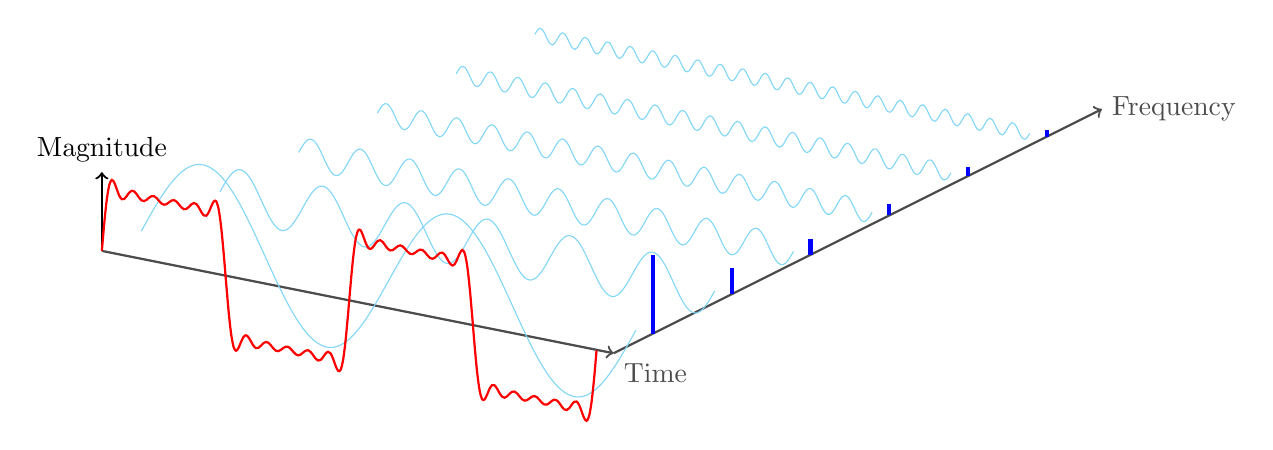
\begin{tikzpicture}[x={(1cm,0.5cm)},z={(0cm,0.5cm)},y={(1cm,-0.2cm)}]%指定坐标系的方向与缩放
            \draw[->,thick,black!70] (0,6.5,0) -- (6.2,6.5,0) node[right] {Frequency}; % 频率轴
            \draw[->,thick,black!70] (0,0,0) -- (0,6.5,0) node[below right] {Time}; % 时间轴
            \draw[->,thick] (0,0,0) -- (0,0,2) node[above] {Magnitude}; 
            
            \foreach \n in {0.5,1.5,...,5.5}{
            \draw [cyan!50, domain=0:2*pi,samples=200,smooth] 
             plot (\n,\x, {sin(4*\n*\x r)/\n });
            \draw[blue, ultra thick] (\n,6.5,0) -- (\n,6.5,1/\n);
            } % 频率逐渐增大振幅逐渐变小的正弦函数
            
            \draw [red, thick, domain=0:2*pi,samples=200,smooth] 
            plot (0,\x, {sin(4*0.5*\x r)/0.5 + sin(4*1.5*\x r)/1.5 + sin(4*2.5*\x r)/2.5
             + sin(4*3.5*\x r)/3.5 + sin(4*4.5*\x r)/4.5 + sin(4*5.5*\x r)/5.5} ); 
            % 最后是手动加起来得到矩形波的逼近
            \end{tikzpicture}
            \caption{测试图1}
        \end{figure}
        
\end{lstlisting}

\begin{figure}[H]

\centering
    
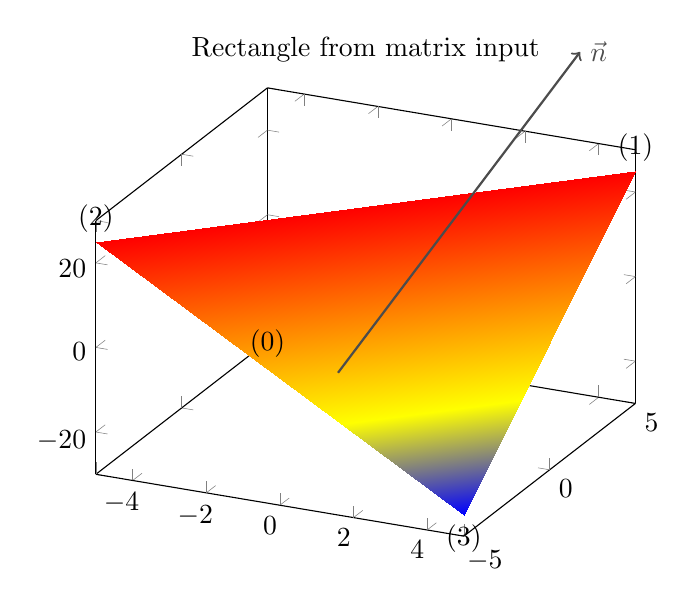
\begin{tikzpicture}
    \begin{axis}[nodes near coords={(\coordindex)},
        title=Rectangle from matrix input]
    % note that surf implies 'patch type=rectangle'
    \addplot3[surf,shader=interp,samples=2,
        patch type=rectangle] 
        {x*y};
    \end{axis}

    \draw[->,thick,black!70] (5,4,5) -- (10,10,10) node[right] {$\vec{n}$};
    

\end{tikzpicture}

\caption{三维绘图}

\end{figure}

\begin{lstlisting}
    
    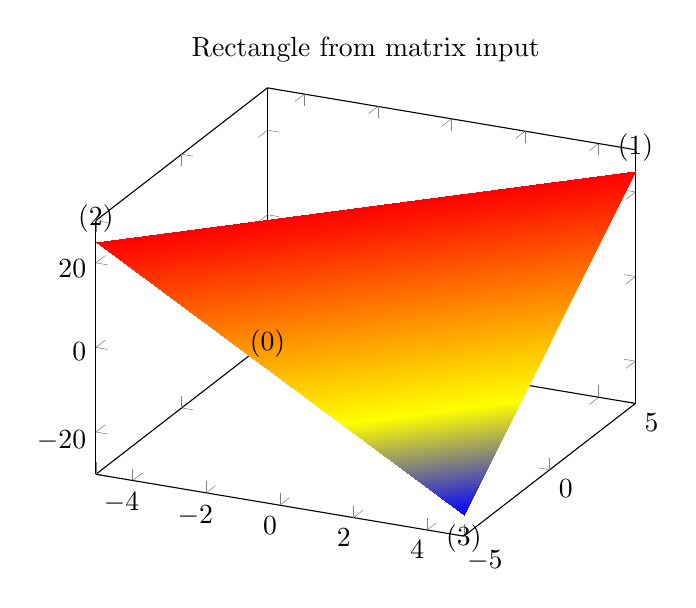
\begin{tikzpicture}
        \begin{axis}[nodes near coords={(\coordindex)},
            title=Rectangle from matrix input]
        % note that surf implies 'patch type=rectangle'
        \addplot3[surf,shader=interp,samples=2,
            patch type=rectangle] 
            {x*y};
        \end{axis}
    \end{tikzpicture}

\end{lstlisting}